%%=============================================================================
%% Methodologie
%%=============================================================================

\chapter{\IfLanguageName{dutch}{Methodologie}{Methodology}}
\label{ch:methodologie}

%% TODO: Hoe ben je te werk gegaan? Verdeel je onderzoek in grote fasen, en
%% licht in elke fase toe welke stappen je gevolgd hebt. Verantwoord waarom je
%% op deze manier te werk gegaan bent. Je moet kunnen aantonen dat je de best
%% mogelijke manier toegepast hebt om een antwoord te vinden op de
%% onderzoeksvraag.

In dit hoofdstuk zal de gebruikte werkwijze van het onderzoek diepgaand uitgelegd worden met de nodige verantwoording.

Dit onderzoek stelt een werkwijze voor om handgeschreven karakters te classificeren per schriftsysteem aan de hand van een convolutioneel neuraal netwerk.
De gebruikte werkwijze bestaat uit verschillende fasen en die komen in dit hoofdstuk aan bod.


\section{Dataverzameling}

De eerste stap in de werkwijze van dit onderzoek was het nagaan welke datasets nodig waren om het model te trainen.
Het doel van het model is om handgeschreven karakters te classificeren per schriftsysteem, hiervoor waren verschillende datasets van meerdere schriftsystemen nodig, deze bestaande uit de afbeeldingen van handgeschreven karakters.

Een grote factor die invloed had op de keuze van de schriftsystemen lag bij de beschikbaarheid van datasets van het schriftsysteem.
Wanneer een potentieel schriftsysteem werd gekozen moest het toeval er bij liggen dat er een dataset bestond waarbij de data bruikbaar was en uit voldoende data bestond.
Als de dataset niet voldeed aan de eisen werd de dataset achterwege gelaten.
Vervolgens werd er of naar een andere dataset gezocht of werd het schriftsysteem niet gebruikt.



Geweten is dat er 3 grote groepen zijn bij de schriftsystemen, het lag voor de hand om één schriftsysteem te gebruiken per groep.

Het eerste schriftsysteem dat voldeed aan de eisen was het Latijns schrift, dit onder de CoMNIST dataset.
De dataset is een online dataset aangezien de data wordt verzameld door middel van een webapplicatie waar iedereen aan kan deelnemen.
Deze dataset bestaat uit twee mappen, één daarvan is het Latijns schrift, de andere is het Cyrillisch schrift dat in dit onderzoek niet gebruikt zal worden.
Het Latijns schrift wordt vooral gebruikt in de westerse wereld, dit is de reden waarom het een eerste en simpele keuze was.
Dit schrift valt onder de alfabetische groep en vult al één van de drie plaatsen op.

De tweede plaats werd opgevuld door het Kanji, één van de schriften gebruikt in het Japans.
Dit schrift valt onder de logografische groep en is daardoor een goede tweede keuze.
De naam van de dataset is de Kuzushiji-MNIST dataset, een offline dataset.
Deze bestaat uit drie verschillende mappen, enkel de Kuzishiji-Kanji werd gebruikt aangezien dit het grootste aantal aan verschillende karakters bevatte.
Dit zou een voordeel bieden voor het trainen van het model.

Voor de laatste plaats werd er een syllabisch schrift gekozen.
Het gekozen schrift was het Arabisch, een gekend lettergrepenschrift dat vooral in de Arabische wereld wordt gebruikt.
Een dataset in het bezit van \autocite{Ahmed2017}, bestaande uit een groot aantal Arabische karakters.

\section{Datavoorbereiding}

Twee van de drie gekozen datasets zijn bedoeld voor het herkennen van de karakters onder het schriftsysteem van de dataset.
Deze datasets bestonden daardoor uit een structuur van mappen waarbij elke map een specifiek karakter voorstelde uit het schriftsysteem, in elke map zaten vervolgens alle afbeeldingen toebehorend aan dat karakter.

Aangezien in dit onderzoek enkel gezocht werd naar het bijhorende schriftsysteem was het voordelig dat alle afbeeldingen in één grote map zaten.
Er werd hier gesproken over meer dan 10.000 afbeeldingen, deze allen verplaatsen met windows file explorer was geen goede keuze.
Voor deze data verplaatsing werd er eens bash script geschreven dat alles verplaatste. (Tabel \ref{table:BashScript})

\begin{table}[!htbp]
    \begin{tabular}{|l|}
        \hline
        \begin{lstlisting}
find . -mindepth 2 -type f -print -exec mv {} . \;
        \end{lstlisting}
        \\ \hline
    \end{tabular}
    \caption{Bash script voor alle data in één map te verplaatsen. }\label{table:BashScript}
\end{table}

Wanneer al de data voldoende was gestructureerd was het klaar voor de manipulaties die nodig waren voor gebruik.

De datamanipulatie werd gedaan in python, hier waren verschillende libraries voor gebruikt, genaamd numpy, matplotlib, os, tqdm en cv2.
Wanneer een model getraind wordt aan de hand van een groot aantal verschillende afbeeldingen moeten de afbeeldingen allen dezelfde afmetingen bevatten, de keuze voor de hoogte en breedte had invloed op het detailgehalte van de afbeelding, wanneer een lage waarde werd gekozen was er weinig detail te zien, bij een grote waarde was er meer detail te zien.
Voor de afmeting van de afbeeldingen die gebruikt werden bij het model werd een waarde van 60 genomen. (Figuur \ref{tab:afmetingen})


\begin{figure}
    
    
    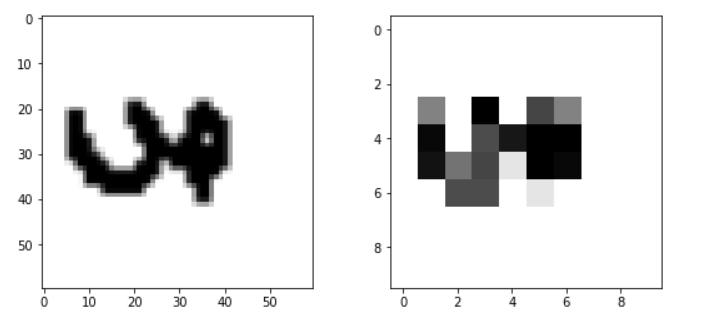
\includegraphics[width=\linewidth]{img/Afmetingen.png}

    \caption{verschil tussen een waarde van 60 (60x60) en een waarde van 10 (10x10) voorgesteld door een Arabisch karakter uit de gebruikte data.}
    \label{tab:afmetingen}
    
\end{figure}

Bij een classificatieprobleem, waar dit onderzoek mee kampt, worden de klassen voorgesteld door numerieke waarden (0, 1, 2, ...). Deze numerieke waarden worden labels genoemd.
Vervolgens worden de afbeeldingen gelinkt aan de bijhorende numerieke waarde.
Bij dit onderzoek zijn de numerieke waarden de schriftsystemen.
Voor het vergemakkelijken voor het model om de data te begrijpen werd er voor gezorgd dat de afbeeldingen allen zwart op wit stonden, de Kanji dataset is bijvoorbeeld wit op zwart dit werd gecorrigeerd.
Als voorlaatste stap werden de afbeeldingen omgezet naar twee-dimensionale matrices waarbij elke waarde in de matrix een waarde voorstelde van de pixel op die positie in de afbeelding.
Uiteindelijk werd de matrix in een lijst geplaatst met de bijhorende label (de numerieke waarde die het schriftsysteem voorstelt). (Tabel \ref{table:DataManipulation})


\begin{table}[!htbp]
    \begin{tabular}{|l|}
        \hline
        \begin{lstlisting}
training_data = []
def create_train_data():
   for category in CATEGORIES: 
      path = os.path.join(DATADIR,category) 
        class_num = CATEGORIES.index(category)
        for img in tqdm(os.listdir(path)): 
          try:
             if(category == "Kanji"):
                 img_array = cv2.imread(
                    os.path.join(path,img),cv2.IMREAD_GRAYSCALE) 
             else:
                 img_array = cv2.bitwise_not(cv2.imread(
                    os.path.join(path,img),cv2.IMREAD_GRAYSCALE))
             new_arr = cv2.resize(img_array,(IMG_SIZE,IMG_SIZE))
             training_data.append([new_arr, class_num])
           except Exception as e:
             pass
        \end{lstlisting}
        \\ \hline
    \end{tabular}
    \caption{Python code voor de manipulatie van de gebruikte datasets (CATEGORIES zijn de gebruikte schriftsystemen) }\label{table:DataManipulation}
\end{table}

De data werd vervolgens willekeurig door elkaar geschud en opgesplitst in twee verschillende lijsten, een lijst van de matrices die de afbeelding voorstelt en een lijst van de bijhorende labels. De positie van een afbeelding in de lijst van matrices ligt op dezelfde positie als de bijhorende label in de andere lijst.
Om de verwerkte data op te slaan werd pickle gebruikt (Tabel \ref{table:DataSave})


\begin{table}[!htbp]
    \begin{tabular}{|l|}
        \hline
        \begin{lstlisting}
import pickle
       
pickle_out = open("X.pickle","wb")
pickle.dump(X, pickle_out)
pickle_out.close()
        \end{lstlisting}
        \\ \hline
    \end{tabular}
    \caption{Het opslaan van de verwerkte data in python door middel van pickle }\label{table:DataSave}
\end{table}

\section{Het Convolutioneel Neuraal Netwerk}

Het ontwerpen van een neuraal netwerk is een proces van trial-and-error.
Een eerste model wordt ontworpen, getraind en als laatste getest, wanneer de accuraatheid van het model niet hoog ligt wordt er gekeken naar het ontwerp van het model.
Er wordt gekeken of er enige aanpassingen nodig zijn voor het verbeteren van de resultaten, wanneer de accuraatheid hoger ligt dan voorheen wordt op dit model verder gewerkt.
Uiteindelijk wordt er een model ontwikkeld dat het best past bij het classificatieprobleem.
In dit hoofdstuk wordt het model besproken dat het best past bij het onderzoek, alsook de verantwoording voor de structuur van het model.

Het model werd ontworpen in python. Voor de implementatie van alle lagen, het laten trainen en testen met de voorbereide data werd tensorflow gebruikt, een open source platform die zich specialiseert in machine learning.
In python werd de library ingeladen zodat de nodige lagen voor een convolutioneel neuraal netwerk gebruikt konden worden.

Aangezien het neuraal netwerk waarden inleest tussen 0 en 1 werden de waarden in de lijst van de lijst van matrices genormaliseerd.
Vervolgens werd de data opgesplitst in traindata waarop het model werd getraind en testdata waarop de accuraatheid van het model werd getest.  \ref{table:DataNormalisition}



\begin{table}[!htbp]
    \begin{tabular}{|l|}
        \hline
        \begin{lstlisting}
X = pickle.load(open("X.pickle","rb"))
y = pickle.load(open("y.pickle","rb"))
       
X = X/255.0

X_train, X_test, y_train, y_test =
       train_test_split(X,y,test_size=0.2)
        \end{lstlisting}
        \\ \hline
    \end{tabular}
    \caption{Het inladen en normaliseren van de data en het opsplitsen van de data} \label{table:DataNormalisition}
\end{table}


Een model wordt aangemaakt en de nodige lagen worden toegevoegd, als eerste laag werd een convolutionele laag geplaatst in het model.
Voor deze laag zijn een aantal parameters nodig, als eerste wordt het aantal filters gevraagd. 
Het aantal filters bepaalt ook het aantal neuronen in de laag, want elke filter is verbonden met een neuron.
De keuze voor het aantal filters ligt bij hoeveel karakteristieken herkend willen worden, aangezien het de eerste laag is werd een aantal van 32 filters gekozen.

Als tweede parameter werd de afmeting gevraagd voor de filter.
De keuze voor de afmeting wordt bepaald door welke soort karakteristieken de filters moeten kunnen verwerken. Wanneer veel detail in de afbeelding aanwezig is zullen kleinere afmetingen worden meegegeven, als grotere karakteristieken moeten herkend worden waar weinig detail aan te pas komt zullen grotere afmetingen worden meegegeven.
Aangezien in de eerste laag vooral simpele karakteristieken zoals vormen, krommingen, et cetera moeten herkend worden werd een afmeting van 5x5 meegegeven.
Als geweten is dat de kleinst mogelijke filter een afmeting van 3x3 bevat zorgt de gekozen afmeting van 5x5 voor het leren van gedetailleerde karakteristieken maar meer rekening houdend met omliggende factoren.

Een derde parameter dat wordt gevraagd is de activatiefunctie, de activatiefunctie bepaalt de uitvoer van de laag.
Voor deze laag werd 'Relu', ook wel 'Rectified linear unit' genoemd, gekozen.

        $f(x) = x^+ = max(0,x)$

Deze functie verandert alle negatieve waarden naar 0 en de positieve waarden blijven hun waarde behouden.
Wanneer deze functie wordt uitgevoerd op een afbeelding blijven enkel de grijze en witte waarden over, de zwarte waarden worden vervangen.
Door deze activatiefunctie wordt het trainingsproces versneld.
(Figuur \ref{tab:Relu})

\begin{figure}
    
    
    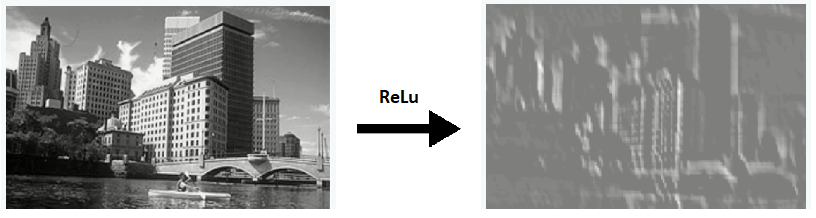
\includegraphics[width=\linewidth]{img/ReLu.png}
    
    \caption{ReLu functie uitgevoerd op een afbeelding.}
    \label{tab:Relu}
    
\end{figure}

Bij de eerste laag in een convolutioneel neuraal netwerk wordt de afmeting gevraagd van de matrices die in de inputlaag zullen worden meegegeven. 

\begin{table}[!htbp]
    \begin{tabular}{|l|}
        \hline
        \begin{lstlisting}
model.add(
    Conv2D(32, (5, 5), activation='relu',input_shape=X.shape[1:]))
model.add(
    MaxPooling2D((2, 2)))

        \end{lstlisting}
        \\ \hline
    \end{tabular}
    \caption{Een eerste convolutioneele laag en een pooling laag}\label{table:FirstLayers}
\end{table}

Nadat een convolutionele laag is toegevoegd aan het model wordt er een pooling laag achter geplaatst.
Bij de pooling laag zijn de verwachte parameters de afmeting van de filters.
Alsook werd deze soort laag toegevoegd aan het neuraal netwerk, 
de gekozen soort pooling laag was een max pooling laag.
Een afmeting van 2x2 werd meegegeven aan de laag.

Een volgende laag dat werd toegevoegd was een convolutionele laag,
een aantal van 64 filters werd gekozen voor deze laag en een afmeting van 7x7.
Het doel van deze laag was het herkennen van grotere patronen met weinig detail, aangezien de vorige laag simpele patronen zou herkennen kon deze laag deze ook gebruiken en zodanig een beter inzicht hebben op de vorm en complexiteit van de karakters.
Net zoals bij de vorige convolutionele laag werd als activatiefunctie ook de Relu functie gekozen.
Vervolgens werd een max-pooling laag toegevoegd met een afmeting van 2x2 voor de filters.

Een derde en laatste convolutionele laag werd nog toegevoegd aan het model met een aantal van 128 filters en een afmeting van 3x3 voor de filters.
Aangezien de afmeting van de filters de kleinst mogelijke waarde bevat staat de laag in voor het herkennen van de details in de karakters.
Deze laag is een belangrijke laag aangezien dit de patronen herkent die eigen zijn aan het schriftsysteem.
Schriftsystemen kunnen onderscheiden worden aan de hand van de kleine details die steeds herkenbaar zijn in de karakters van het schriftsysteem.
Daarom werd een hoog aantal filters meegegeven aan deze laag, zodanig dat de vele details eigen aan de karakters en specifiek aan het schriftsysteem kunnen herkend worden.
Uiteindelijk werd nog een max-pooling laag geplaatst in het model met een afmeting van 2x2 voor de filters.

De convolutionele lagen staan in voor het herkennen van de karakteristieken en patronen, vooraleer een schatting kan verkregen worden van het toebehorende schriftsysteem moeten er nog enkele normale lagen worden toegevoegd.
Er werd gewenst om de uitvoer van de convolutionele lagen in te voeren in normale lagen.
Een convolutioneel neuraal netwerk werkt met invoer in de vorm van 2-dimensionale lijsten.
Een normaal neuraal netwerk daarentegen kan hier niet mee werken, vooraleer de uitvoer van een convolutionele laag in een normale laag kan worden ingevoerd moeten de matrices, 2-dimensionale lijsten, omgevormd worden naar lijsten met 1 dimensie.
Voor deze operatie bestaat er een specifieke laag, de flatten laag.
Na de convolutionele lagen werd zo een dergelijke laag toegevoegd.

Bij een normale laag of dense laag worden ook een aantal parameters gevraagd, waarvan de eerste het aantal neuronen verwacht en de tweede de activatiefunctie verwacht.

Een eerste normale laag werd toegevoegd met een aantal van 128 neuronen en als activatiefunctie werd de ReLu functie gekozen.
Bij deze laag werd een hoog aantal neuronen gekozen aangezien het in staat voor vele karakteristieken en patronen te linken met het toebehorende schriftsysteem.

Een tweede normale laag werd vervolgens toegevoegd aan het model met een aantal van 64 neuronen en als activatiefunctie werd de ReLu functie gekozen.
Deze laag kreeg een normaal aantal neuronen voor de laatste schattingen uit te voeren op de data.

Een probleem dat zich kan vormen in een neuraal netwerk is overfitting,
overfitting is een fenomeen dat zich voor kan doen wanneer een neuraal netwerk zich te veel focust op een specifieke dataset.
Het model zal een goede voorspelling maken op data uit de meegegeven dataset maar wanneer data wordt meegegeven dat het model nog nooit gezien heeft zal het een veel slechtere voorspelling teruggeven.
Om dit probleem tegen te gaan kan een extra laag worden toegevoegd genaamd de dropout laag.
Deze laag doet het volgende, wanneer een model wordt getraind heeft een neuron een kans om gedeactiveerd te worden.
Dit wil zeggen dat het de taak die het neuron op zich heeft niet meer zal uitvoeren.
Dit zorgt voor 'noise', irregulariteit in trainingsproces.
Wanneer een neuron gedeactiveerd wordt neemt een ander neuron de taak op van het inactieve neuron, hierdoor zal het model meer robuuste karakteristieken kunnen aanleren.
Een dropout-laag verwacht een enkele parameter; de kans dat een neuron gedeactiveerd kan worden.
Aan het netwerk werd een dropout-laag toegevoegd met een waarde van 0.1 voor de kans.

De laatste laag van een neuraal netwerk is steeds de uitvoerlaag.
Als uitvoerlaag bij het netwerk werd een normale laag toegevoegd met drie neuronen, een neuron per schriftsysteem.
Voor de activatiefunctie werd de softmax functie gekozen, de softmax functie geeft aan elk neuron een probabiliteit voor elk schriftsysteem.

Wanneer alle lagen waren toegevoegd werd het model gecompileerd en werden nog drie parameters meegegeven.
Een daarvan was de loss functie, dit is de functie die de loss berekend van bij het trainen van een model.
De loss is het aantal fouten die gemaakt worden bij het trainen, het type loss functie die gebruikt wordt hangt af van welk probleem er getracht opgelost te worden met het ontworpen neurale netwerk.
Hier werd als loss functie de 'sparce categorical crossentropy' gekozen, dit aangezien de schriftsystemen verschillende klassen of categorieën voorstellen.\\
Een volgende parameter die gevraagd werd is de optimalisatie functie, deze functie zorgt ervoor dat de gemaakte loss bij een trainingsproces zo laag mogelijk is, dit doet het door de leerbare parameters aan te passen in het neurale netwerk.\\
De laatste parameter die wordt verwacht is de 'metrics', dit zijn waarden die een ontwerper van een model wil dat ze worden weergegeven bij het trainen van het model. ( Tabel \ref{table:Compile})


\begin{table}[!htbp]
    \begin{tabular}{|l|}
        \hline
        \begin{lstlisting}
        model.compile(loss='sparse_categorical_crossentropy',
                      optimizer='adam',
                      metrics=['accuracy'])
        
        \end{lstlisting}
        \\ \hline
    \end{tabular}
    \caption{Het compileren van het model met de nodige instellingen} \label{table:Compile}
\end{table}

\section{Trainen en testen}

Nadat het model gecompileerd was kon er gestart worden met het trainen van het model, hiervoor werd ook tensorflow gebruikt.
Vooraleer het model werd aangemaakt en de nodige lagen waren toegevoegd werd de lijst van data en labels opgesplitst in trainingsdata en trainingslabels en in testdata en testlabels.
Bij het trainen van een model worden de trainingsdata en de trainingslabels meegegeven.
Vervolgens wordt een batch grootte meegegeven die bepaalt hoeveel data het moet testen per keer, het aantal generaties en een splitsing van de data waarbij het opgesplitste deel gebruikt wordt voor validatie.
De validatie zorgt voor een goedkeuring van de data die getraind wordt.
Hier bij het model kreeg de batch grootte een waarde van 32, het werd getraind over 5 generaties en een derde van de data werd gebruikt voor validatie. ( Tabel \ref{table:Training})



\begin{table}[!htbp]
    \begin{tabular}{|l|}
        \hline
        \begin{lstlisting}
       model.fit(X_train, y_train, batch_size=32,
                 epochs=5,validation_split=0.3)
        \end{lstlisting}
        \\ \hline
    \end{tabular}
    \caption{Het trainen van het model met de nodige parameters} \label{table:Training}
\end{table}

\section{Resultaten}

Wanneer het model zijn generaties had voltooid kon gekeken worden naar de accuraatheid en de loss van elke generatie.
De eerste generatie had al een hoge accuraatheid met een waarde van 0.9703 en een lage loss met een waarde van 0.0757.
Bij elke generatie verhoogde de accuraatheid en verlaagde de loss, zoals verwacht.
De laatste generatie had een accuraatheid met een waarde van 0.9993 en een loss met een waarde van 0.0031.
Dit is een hoge accuraatheid en zal zorgen voor een vloeiend onderscheid bij het onderscheiden van de drie schriftsystemen.
Uiteindelijk werd een laatste evaluatie uitgevoerd met de ongeziene testdata en testlabels.
Ook hier was er een hoge accuraatheid van 0.9996 en een lage loss. ( Figuur \ref{tab:testResults})

\begin{figure}
    
    
    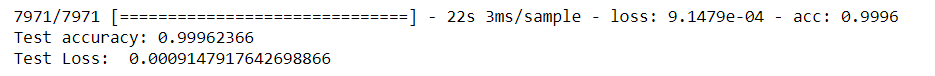
\includegraphics[width=\linewidth]{img/testResults.png}
    
    \caption{Resultaten van de test met weergegeven accuraatheid en loss}
    \label{tab:testResults}
    
\end{figure}

\section{Gebruik}

Een aantal ongekende afbeeldingen werden vervolgens gebruikt met als doel een voorbeeld te geven hoe het gebruikt zou worden in de praktijk.
Een ongekende afbeelding wordt opgeslagen en vervolgens in het model geplaatst.
Eerst en vooral wordt de afbeelding gevormd naar de verwachte afmetingen.
Het model berekent welk schriftsysteem het best past bij de afbeelding en hieruit haalt een script de hoogste waarde uit de lijst van percentages die verkregen zijn vanuit de uitvoerlaag van het model.
Uiteindelijk kijkt het gebruikte script naar de overeenkomende waarde met de lijst van schriftsystemen en geeft dit weer.
De resultaten zijn steeds correct, bij elke afbeelding van een karakter uit een gebruikt schriftsysteem voorspelt het model het juiste schriftsysteem. (Figuur \ref{tab:examples} )

Het gebruik van deze software zou het meest efficiënt zijn met het gebruik van een bijkomende applicatie op een smartphone.
Bij de volgende probleemstelling wordt voorop vastgesteld dat een volledig model is ontwikkeld dat in staat is om een groot aantal veel gebruikte schriftsystemen van elkaar te onderscheiden. \\
Stel nu dat een geleerde in de forensische letterkunde een opdracht krijgt waarbij hij/zij een document dat geschreven is in een ongekend schriftsysteem moet herkennen en lokaliseren. Vooraleer de letterkundige uit eigen ervaring tracht het schriftsysteem te lokaliseren gebruikt hij eerst de mobiele applicatie op zijn smartphone, hij neemt een foto van een karakter in het document en krijgt vervolgens een voorspeld resultaat. \\
Hiervoor moet de software niet volledig accuraat zijn, aangezien het een ongekend schriftsysteem is zal het ook niet veel gebruikt zijn en bestaat de kans dat het niet aangeleerd is aan het model.
Maar een ongekend schriftsysteem dat niet veel gebruikt wordt stamt vaak af van een ander schriftsysteem waarbij de kans wel bestaat dat het aangeleerd is aan het model. \\
Wanneer de mobiele applicatie het schriftsysteem teruggeeft dat veel eigenschappen deelt met het ongekende schriftsysteem, geeft dit al een goede start aan de letterkundige voor het lokaliseren van het ongekende schrift.

Wanneer gewerkt zou worden met volledige woorden of paragrafen bestaande uit karakters uit een schriftsysteem zouden alle karakters herkend kunnen worden en een pluspunt geven aan het door het model voorspelde schriftsysteem.
Als voor alle karakters een voorspelling is gemaakt zou het schriftsysteem met de meeste pluspunten gekozen worden als resultaat.

 
\begin{figure}
    
    
    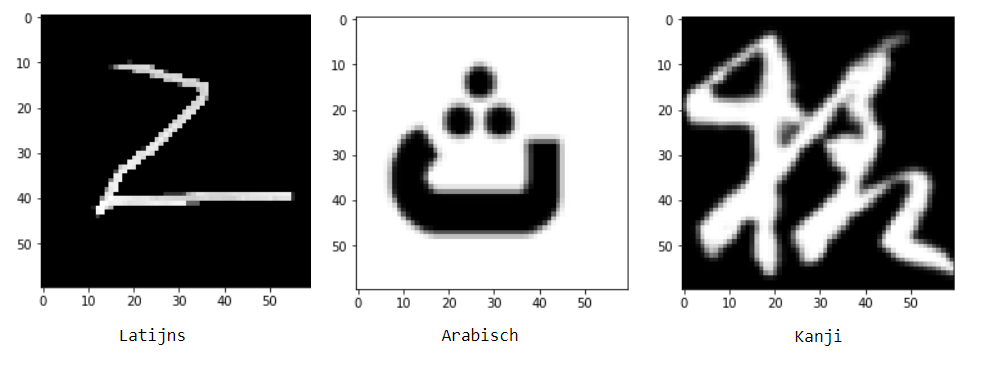
\includegraphics[width=\linewidth]{img/voorbeelden.png}
    \caption{Voorbeelden van het model in de praktijk}
    \label{tab:examples}

\end{figure}









 














